\documentclass[Cursovd_portada.tex]{subfiles}
\begin{document}

\chapter{Aplicación Diferencial de una\\ Aplicación
Diferenciable}
 \hs La definición de espacio tangente en cada
punto de una variedad diferenciable y, por tanto, la idea de
``aproximar" la variedad en el punto por un espacio vectorial,
permite, a su vez, dada una aplicación diferenciable entre dos
variedades diferenciables, definir la noción de diferencial de
tal aplicación en cada punto de la variedad dominio como una
aplicación lineal entre los espacios tangentes del punto y del
punto imagen, que generaliza a la bien conocida entre espacios
euclídeos. El conocimiento de las propiedades de tales
aplicaciones es de gran utilidad, pues están directamente
relacionadas con la naturaleza diferenciable de la aplicación
de partida.
\section{Aplicación Diferencial y Aplicación Co\-di\-fe\-ren\-cial de una Aplicación Diferenciable.}
\begin{defi}
Sean $M$ y $N$ dos variedades diferenciables, $f\in\mathcal{F}(M,N)$ y $p\in M$. Se llama {\bf Diferencial} de $f$
en $p$ a la aplicación $f_{*p}:T_p(M)\fl T_{f(p)}(N)$ definida de la siguiente forma: si $u\in T_p(M)$ es
cualquier vector tangente a $M$ en $p$ y $\a:(a,b)\fl M$ es una curva diferenciable que pasa por $p$ y cuyo vector
tangente en $p$ es $u$ (es decir, si existe $t_0\in (a,b)$ con $\a(t_0)=p$ y $\a'(t_0)=u$), entonces
$f_{*p}u=(f\circ\a)'(t_0)$.
\end{defi}
Obsérvese que, desde luego, $f_{*p}u$ es un vector tangente a $N$ en $f(p)$, pues $f\circ\a:(a,b)\fl N$ es una
curva diferenciable en $N$, que pasa por $f(p)$, ya que $f(\a(t_0))=f(p)$ y, por tanto, $(f\circ\a)'(t_0)\in
T_{f(p)}(N)$. Además, la definición anterior no depende de la curva $\a$ elegida pasando por $p$ y con vector
tangente en $p$ igual a $u$. En efecto, si $\b:(c,d)\fl M$ es otra curva en las mismas condiciones, entonces
existe $\tau_0\in(c,d)$ tal que $\b(\tau_0)=p$ y $\b'(\tau_0)=u$. Es claro que $f\circ\b:(c,d)\fl N$ es una curva
diferenciable que pasa por $f(p)$, ya que $(f\circ\b)(\tau_0)=f(p)$ y su vector tangente en $f(p)$ es $f_{*p}u$,
pues dada cualquier $g\in\mathcal{F}(f(p))$, se tiene que:
$$(f\circ\b)'(\tau_0)g=\left.\dderi{(g\circ(f\circ\b))}{\tau}\right|_{\tau=\tau_0}=
\left.\dderi{((g\circ f)\circ\b)}{\tau}\right|_{\tau=\tau_0}=$$
$$=\b'(\tau_0)(g\circ f)=u(g\circ f)=\a'(t_0)(g\circ f)=$$
$$=\left.\dderi{((g\circ f)\circ\a)}{t}\right|_{t=t_0}=\left.\dderi{(g\circ(f\circ\a))}{t}\right|_{t=t_0}=
(f\circ\a)'(t_0)g=(f_{*p}u)g.$$
\begin{prop}
Si $f\in\mathcal{F}(M,N)$, $p\in M$, $u\in T_p(M)$ y $g\in\mathcal{F}(f(p))$, entonces se verifica:
$$(f_{*p}u)g=u(g\circ f).$$
\end{prop}
\begin{prop}
{\bf (Propiedades de la Diferencial).}
\begin{enumerate}
\item {\bf (Regla de la Cadena).} Sean $f\in\mathcal{F}(M,N)$ y $g\in\mathcal{F}(N,P)$. Entonces, para
cualquier $p\in M$ se verifica que $(g\circ f)_{*p}=g_{*f(p)}\circ f_{*p}$.
\item Dado $p\in M$, entonces $({\rm Id}_M)_{*p}={\rm Id}_{T_p(M)}$.
\item Si $f,g\in\mathcal{F}(M,N)$ y $f\equiv g$ en un entorno de $p\in M$, entonces $f_{*p}=g_{*p}$.
\end{enumerate}
\end{prop}
\begin{dem}
\begin{enumerate}
\item[]
\item $\forall h \in G(g(f(p))$ tenemos que 
\begin{gather*}
((g\circ f)_{\ast p}u)h = u(h\circ(g \circ f)) = u ((h\circ g) \circ f) = (f_{\ast p}(h \circ g)) = (g_{\ast f(p)}(f_{\ast p} u))h
\end{gather*}
\item $\forall h \in G(p)$ $((id_M)_{\ast p}h = u(h \circ id_M) = u(h)$
\item $\forall u \in T_p(M)$ y $\forall h\in F(f(p))$ tenemos que 
\begin{gather*}
(f_{\ast p}u)h = u(h\circ f)=u(h \circ g) = (g_{\ast p} u)h
\end{gather*}
Por tanto, $f_{\ast p}u=g_{\ast p}u$ $\forall u$.
\end{enumerate}
\end{dem}
\begin{prop}
La diferencial en cada punto de una aplicación diferenciable es una aplicación lineal.
\end{prop}
\begin{dem}
Veámoslo directamente $\forall g\in F(f(p))$
\begin{gather*}
 f_{\ast p}(\lambda u+\mu v)g = (\lambda u+\mu v)(g\circ f)= \lambda u(g \circ f)+\mu v(g \circ f) = (\lambda f_{\ast p} u + \mu f_{\ast p})g
\end{gather*}
\end{dem}
En consecuencia, cada diferencial tiene asociada una matriz. Para calcularla, sean $(U,\vp=(x_1,\dots ,x_m))$ un
s.l.c. de $M$ entorno de $p$ y $(V,\psi=(y_1,\dots ,y_n))$ un s.l.c. de $N$ entorno de $f(p)$. Para estas cartas
locales, las bases de $T_p(M)$ y $T_{f(p)}(N)$ son
$$\left\{\left(\dep{x_1}\right)_p,\dots ,\left(\dep{x_m}\right)_p\right\}\mbox{ }{\rm y}\mbox{
}\left\{\left(\dep{y_1}\right)_{f(p)},\dots ,\left(\dep{y_n}\right)_{f(p)}\right\},$$ respectivamente. Entonces,
como
$$f_{*p}\left(\dep{x_i}\right)_p=\sum_{j=1}^n\left[f_{*p}\left(\dep{x_i}\right)_p(y_j)\right]\left(\dep{y_j}
\right)_{f(p)}=$$ $$=\sum_{j=1}^n\left[\left(\ddep{(y_j\circ f)}{x_i}\right)_p\right]\left(\dep{y_j}
\right)_{f(p)},$$ la matriz de $f_{*p}$ respecto de estas bases viene dada por
$$f_{*p}=\left[\left(\ddep{y_j\circ f}{x_i}\right)_p\right],$$
que es la matriz jacobiana de la aplicación $\psi\circ f\circ\vp^{-1}:\vp(U\cap f^{-1}(V))\fl\psi(f(U\cap
f^{-1}(V)))$.
\begin{defi}
La matriz anterior se denomina {\bf Matriz Jacobiana} de $f$ en $p$ respecto de las cartas dadas. En el caso en
que ${\rm dim}(M)={\rm dim}(N)$, el determinante de esta matriz se llama {\bf Jacobiano} de $f$ en $p$ y se denota
por $J_p(f)$.
\end{defi}
\begin{prop} Si $f\in\mathcal{F}(M,N)$, siendo $M$ conexa y $f_{*p}=0$, para cual\-quier $p\in M$, entonces $f$
es constante.
\end{prop}
\begin{dem}
Sean $p\in M$ y $q=f(p)\in N$. Entonces $A=f^{-1}(\{q\})\neq\emptyset$. Además, $A$ es cerrado por continuidad de $f$ en un espacio T1. Veamos que $A$ es abierto para probar que $A=M$. Sea $\overline{p}\in A$ arbitrario tal que $f(\overline{p})=q$. Sean $(U,\varphi=(x_1,\dots,x_n))$ carta en $M$ tal que $\overline{p}\in U$ y $(V,\psi=(y_1,\dots,y_n))$ en $N$ tal que $q\in V$. Podemos suponer que $U$ es conexo pues en caso contrario bastaría tomar una de sus componentes conextas, y $f(U)\subseteq V$. Así, $\forall \tilde{p}\in U,\ \forall i=1,\dots, m$ $f_*\left(\frac{\partial}{\partial x_i}\right)_{\tilde{p}}=0\in T_{f(\tilde{p})}(N)$. En particular, $f_*\left(\frac{\partial}{\partial x_i}\right)_{\tilde{p}}y_j=0\ \forall j=1,\dots, n$, es decir, 
$$\left.\frac{\partial(y_j\circ f)}{\partial x_i}\right|_{\tilde{p}}=\left.\frac{\partial(u_j\circ\psi\circ f\circ\varphi^{-1})}{\partial u_i}\right|_{\varphi(\tilde{p})}$$
Al ser $\varphi(U)$ conexo, exto implica que $\psi\circ f\varphi^{-1}$ es constante, luego en particular, $\forall \tilde{p}\in U$, 
$$\psi(f(\tilde{p}))=\psi\circ f\varphi^{-1}(\varphi(\tilde{p}))=\psi\circ\varphi^{-1}(\varphi(\overline{p}))=\psi(f\overline{p}))=\psi(q)$$
Por la inyectividad de $\psi$, $f(\tilde{p})=q$, luego $U\subseteq f^{-1}(\{q\})=A$. Esto implica que todo punto de $A$ es interior y por tanto $A$ es abierto, como queríamos demostrar. $\QED$
\end{dem}

\begin{defi}
Una aplicación $f\in\mathcal{F}(M,N)$ se dice que es {\bf No Singular} en $p\in M$ si $f_{*p}$ es inyectiva, es
decir, si $\ker f_{*p}=0$. Al rango (dimensión de la imagen) de $f_{*p}$ se le denomina {\bf Rango} de $f$ en $p$.
El punto $p$ se dice {\bf Regular} para $f$ si $f_{*p}$ es sobreyectiva. En caso contrario, $p$ se dice {\bf
Crítico}. Si $p$ es crítico para $f$, el punto $q=f(p)$ se denomina {\bf Valor Crítico}. De lo contrario se llama
{\bf Valor Regular}.
\end{defi}
Obsérvese que si ${\rm dim}(M)={\rm dim}(N)$, entonces $p\in M$ es regular para $f$ si y sólo si $f_{*p}$ es un
isomorfismo, es decir, si y sólo si $J_p(f)\neq 0$.
\begin{defi}
Una aplicación $f\in\mathcal{F}(M,N)$ se dice que es una {\bf Inmersión} si es no singular en todos los puntos de
$M$, es decir, si su diferencial en cada punto es una aplicación inyectiva y se dice que es una {\bf Sumersión} si
todos los puntos de $M$ son regulares para $f$, es decir, si su diferencial en cada punto es una aplicación
sobreyectiva.
\end{defi}
\begin{defi}
Sea $f\in\mathcal{F}(M,N)$ y $p\in M$. Se llama {\bf Aplicación Co\-di\-fe\-ren\-cial} de $f$ en $p$ a la
aplicación dual de $f_{*p}$, denotada por $f_p^*$ y dada por
$$f_p^*:T_{f(p)}^*(N)\fl T_p^*(M):\om\mapsto f_p^*\om$$
tal que, para cualquier $u\in T_p(M)$, $(f_p^*\om)u=\om(f_{*p}u)$.
\end{defi}
\begin{prop}
{\bf (Regla de la Cadena de la Codiferencial).} Sean $f\in\mathcal{F}(M,N)$, $g\in\mathcal{F}(N,P)$ y $p\in M$.
Entonces, se verifica que $(g\circ f)_p^*=f_p^*\circ g_{f(p)}^*$.
\end{prop}
\begin{dem}
Sea $u^*\in T^*_{g(f(p))}(P)$ y $v\in T_p(M)$.  $$((g\circ f)^*_p u^*)v=u^*((g\circ f)_{*p}v)=u^*(g_{*f(p)}\circ (f_{*p}v))=(g^*_{f(p)}u^*)(f_{*p}v)=(f^*_p(g^*_{f(p)}u^*))v$$ $\QED$
\end{dem}

\begin{dem}
Para todo $u^* \in T^*_{g(f(p))}$ y todo $v \in T_p(M)$:
\[ ((g \circ f)^*_p u^*)v = u^*((g \circ f)_{*p} v) \]
Aplicando la regla de la cadena:
\[ ((g \circ f)^*_p u^*)v = u^*( g_{*f(p)} (f_{*p}(v))) = (g_{f(p)}^*u^*) (f_{*p} v) = (f_p^*(g_{f(p)}^*u^*))v\]
Luego $(g \circ f)^*_p  = f_p^* \circ g_{f(p)}^*$.
\end{dem}

\subsubsection{Recordatorio Álgebra Lineal}

Dada $F:V\to W$ lineal, con bases en cada espacio $B_1=\{v_1,\dots,v_m\}$ y $B_2=\{w_1,\dots,w_m\}$, y matriz $M_{B_1,B_2}(F)=A=(a_{ij})$, entonces $Fv_i=\sum_{j=1}^m a_{ij}w_j$. Tomando la aplicación dual obtenemos $F^*:W^*\to V^*$, $B_2^*=\{w^*_1,\dots,w^*_m\}$, $B_1^*=\{v^*_1,\dots,v^*_m\}$ tales que $w^*_i(w_j)=\delta_{ij}$ y $v^*_i(v_j)=\delta_{ij}$, con $M_{B^*_1,B^*_2}(F^*)=B=(b_{ij})$, de modo que $F^*w^*_j=\sum_{j=1}^m b_{ji}v_i^*$. Como $(F^*w^*)v=w^*(Fv)$

$$(F^*w^*_j)v_k=\sum_i b_{ji}v^*i(v_k)=b_{jk}$$
$$w^*_j(Fv_k)=w^*_j(\sum_{j=1}^ma_{ki}w_i)=\sum_i a_{ki}w^*_j(w_i)=a_{kj}$$
Luego $B=A^t$. 

\begin{prop}
Sean $f\in\mathcal{F}(M,N)$ y $p\in M$. Entonces, se verifican:
\begin{enumerate}
\item $f_{*p}$ es inyectiva si y sólo si $f_p^*$ es sobreyectiva.
\item $f_{*p}$ es sobreyectiva si y sólo si $f_p^*$ es inyectiva.
\end{enumerate}
\end{prop}

\begin{dem}
La inyectividad y la sobreyectividad dependen de que el rango de la matriz de la transformación tenga rango máximo. Como el functor es contravariante, las dimensión del espacio de llegada se intercambia con la del de salida y recíprocamente, y de ahí el resultado. $\QED$
\end{dem}
\newpage

\section{Noción de Subvariedad.}
\hs La mayoría de los ejemplos familiares de variedades
diferenciables son subconjuntos de otras variedades (puede
pensarse en los abiertos de una variedad diferenciable, las
superficies re\-gu\-la\-res en $\R^3$ o la figura ocho en $\R^2$).
Cabe preguntarse cuándo la estructura diferenciable del
subconjunto viene ``inducida" de alguna manera por la de la
variedad ambiente y cuál es la relación entre ambas
estructuras. Esta relación tiene que ver con el hecho de que
el espacio tangente a la variedad subconjunto sea subespacio del
espacio tangente de la variedad ambiente en cada punto. Aparece
así la noción de subvariedad.
\begin{defi}
Una {\bf Subvariedad} de una variedad diferenciable $N$ es un par $(M,f)$, donde $M$ es otra variedad
diferenciable y $f\in\mathcal{F}(M,N)$ es una inmersión inyectiva.
\end{defi}
En los ejemplos antes mencionados (subvariedades abiertas,
superficies re\-gu\-la\-res o la figura ocho con cualquiera de las
dos estructuras conocidas), la inmersión inyectiva que las
convierte en subvariedad es la inclusión. Sin embargo, esto no
siempre ocurre. Por ejemplo, considérese el intervalo abierto
$(-1,1)$ dotado de la estructura diferenciable dada por la carta
global $\vp(t)=t^3$. Se tiene que $(-1,1)$ es un subconjunto de
$\R$ con la estructura euclídea y la inclusión
$i:(-1,1)\hookrightarrow\R$ no es una inmersión, pues ni
siquiera es diferenciable. Con todo, el par $((-1,1),f)$, con
$f:(-1,1)\fl\R$ la inmersión $f(x)=x^3$ sí es una
subvariedad de $\R$.
\begin{prop}\label{prop}
Sea $(M,f)$ una subvariedad de la variedad diferenciable $N$.
Entonces, puede dotarse a $f(M)$ de una estructura de variedad
diferenciable tal que $(f(M),i)$, con $i:f(M)\hookrightarrow N$ la
inclusión, es una subvariedad de $N$.
\end{prop}
\begin{dem} Observemos el siguiente diagrama
\[
\begin{tikzcd}
p\in M\arrow[r,"f"]\arrow[d,"\overline{f}"'] & q\in N\\
q=f(p)\in f(M)\arrow[ur,"i"'] 
\end{tikzcd}
\]
Usando el problema 2.5 sabemos que $\exists!$ estructura de variedad diferenciable sobre $f(M)$ tal que $f$ es difeomorfismo. Veamos que $(f(M),i)$ es subvariedad de $N$. Primeramente, $f(M)$ es variedad diferenciable, donde $\dim f(M)=\dim M$. Además, $i$ es siempre una función inyectiva y, por composición, $i\in F((f(M),N)$, pues $ i = f \circ (\overline{f})^{-1}$. Además, $i_{\ast q} = f_{\ast (\overline{f})^{-1}(q)}\circ (\overline{f})^{-1}_{\ast q}$.

\end{dem}
Obsérvese que, en el resultado anterior, la topología de $f(M)$ es, en general, más fina que la topología relativa
inducida por la de $N$, pues la inclusión, al ser diferenciable, es continua. Esto lleva a pensar que la noción de
subvariedad es más sutil que la análoga para espacios topológicos. En efecto, como ya se ha dicho, el ocho con
cualquiera de las dos estructuras conocidas es subvariedad de $\R^2$ con la inclusión como inmersión inyectiva y,
sin embargo, no es subespacio topológico de $\R^2$ en ninguno de los dos casos.
\begin{defi}
Se dice que una aplicación $f\in\mathcal{F}(M,N)$ es una {\bf In\-crus\-ta\-ción} si es un homeomorfismo sobre su
imagen, dotada ésta de la topología relativa de $N$, es decir, si $f:M\fl f(M)\subseteq N$ (dando a $f(M)$ la
topología relativa de $N$) es una aplicación biyectiva, continua y abierta o cerrada. \end{defi}
\begin{defi}
Una subvariedad $(M,f)$ de una variedad diferenciable $N$ se dice que es una {\bf Subvariedad Regular} si $f$ es,
además, una incrustación.
\end{defi}
Por tanto, para subvariedades regulares, las imágenes de éstas por la inmersión, dotadas de la estructura dada por
la Proposición \ref{prop}, son también subespacios topológicos de la variedad ambiente. En el caso particular de
considerar subvariedades que sean subconjuntos con la inclusión, se obtiene:
\begin{prop}
Sean $M\subseteq N$ dos variedades diferenciables tales que, si $i:M\hookrightarrow N$ es la inclusión, $(M,i)$ es
subvariedad de $N$. Entonces, $(M,i)$ es subvariedad regular de $N$ si y sólo si $M$ tiene la topología relativa
de $N$.
\end{prop}
\begin{dem}
$id$ es homomorfimo si y solo si $T_M = T_{N}|_M$.
\end{dem}
\section{El Teorema de la Función Inversa.}
\hs Dada una subvariedad $(M,f)$ de una variedad diferenciable
$N$, si ${\rm dim}(M)={\rm dim}(N)$, la diferencial de $f$ en cada
punto de $M$ es un isomorfismo de espacios vectoriales. Este hecho
ocurre, en particular, si $f$ es un difeomorfismo,
verificándose que dos variedades diferenciables difeomorfas
son, cada una de ellas, subvariedad de la otra con inmersión
el difeomorfismo o su inverso, según el caso.
\par Cabe preguntarse, entonces, por el recíproco de este resultado: Dada una subvariedad de una variedad
diferenciable, ambas de la misma dimensión, ?`son difeomorfas
a través de la inmersión? Más en general, si una
aplicación diferenciable entre variedades diferenciables
cumple que su diferencial en cada punto es un isomorfismo, ?`es un
difeomorfismo? La respuesta es negativa, pues basta considerar una
subvariedad abierta de una variedad diferenciable (aquí la
inmersión es la inclusión, que no es un difeomorfismo, al
no ser sobreyectiva).
\par Sin embargo, sí puede probarse, mediante el Teorema de la Función Inversa en Variedades, que una tal aplicación
es un difeomorfismo local. De este teorema se deducen importantes
colorarios sobre las carta locales de ambas variedades. Por otra
parte, la condición adicional que debe impornerse a la
aplicación para que sí sea un difeomorfismo es la
biyectividad.
\begin{teorema}
{\bf (Teorema de la Función Inversa en $\R^m$).} Sean
$G\subseteq\R^m$ un abierto, $f:G\fl\R^m$ una aplicación
diferenciable y $p\in G$ tal que
$$\left|\left(\ddep{(u_i\circ f)}{u_j}\right)_{p}\right|\neq 0.$$
Entonces, existe un abierto $U$, con $p\in U\subseteq G$, tal que
$f(U)$ es abierto de $\R^m$ y $f|_U:U\fl f(U)$ es un
difeomorfismo.
\end{teorema}
\begin{teorema}
{\bf (Teorema de la Función Inversa en Variedades).} Sean
$f\in\mathcal{F}(M,N)$ y $p\in M$ tal que $f_{*p}$ es un
isomorfismo. Entonces, existe un abierto $U$, con $p\in U\subseteq
M$, tal que $f(U)$ es abierto de $N$ y $f|_U:U\fl f(U)$ es un
difeomorfismo.
\end{teorema}
\begin{dem}
\begin{figure}[htp]
\centering
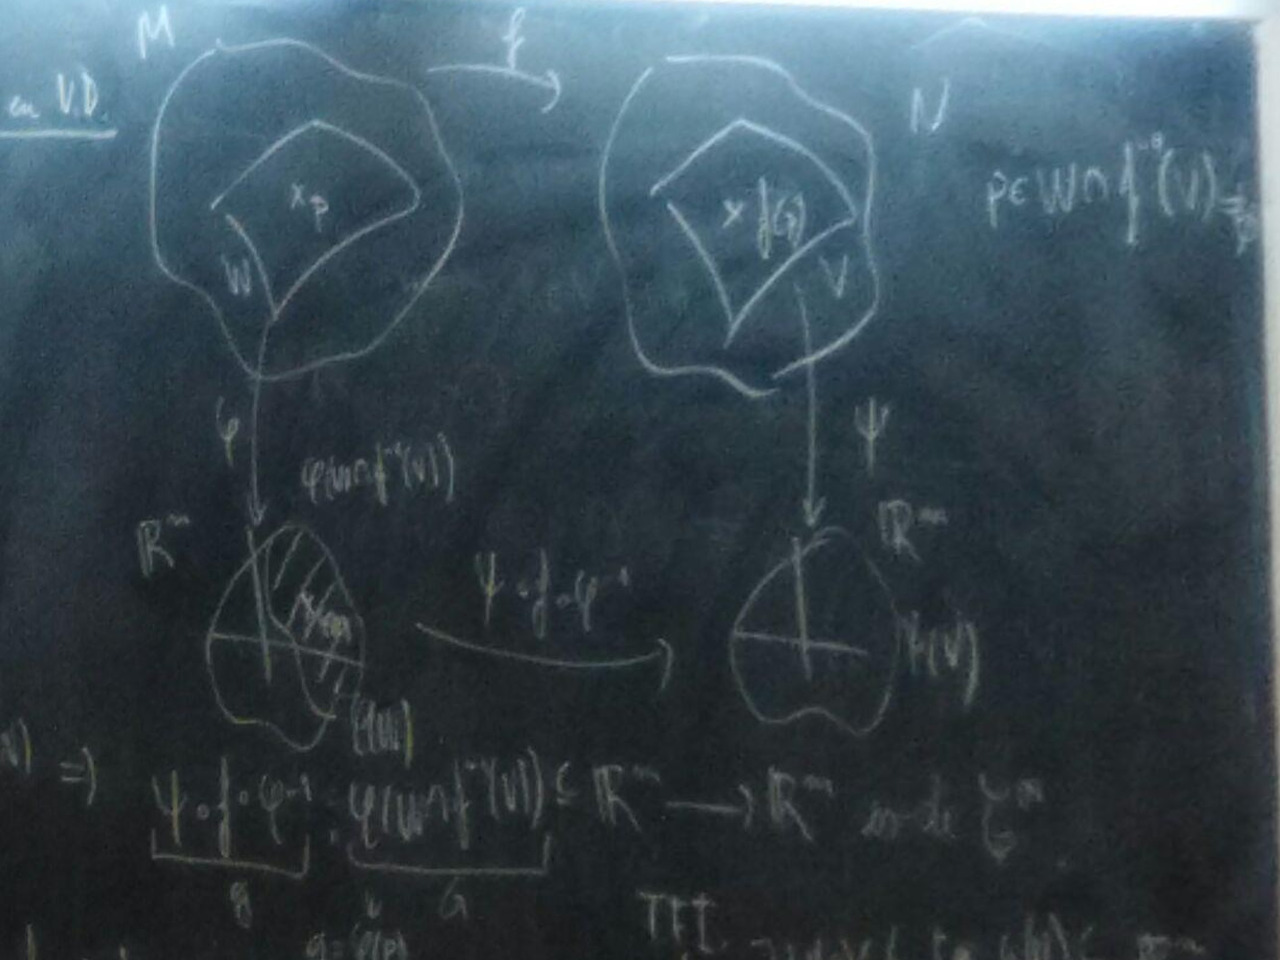
\includegraphics[width=200px]{images/funcioninversa1.jpg}
\caption{}
\label{}
\end{figure}
Llamaos $G = φ(W \cap f^{-1}(V))$. Como $f \in F(M,N)$, entonces $ψ \circ f \circ φ^{-1} : G \to \R^m$ es de $C^{∞}$. Se $g = ψ \circ f \circ φ^{-1}$. Como $f_{*p}$ es isomorfismo, la determinante jacobiano en $φ(p)$ de $g$ es no nulo. Aplicando el teorema de la función inversa en $\R^m$ existe un entorno $H$ de $q$ en $G$ tal que $g(H)$ es abierto en $\R^m$ y $g|_H : H \to g(H)$ es un difeomorfismo.

Sea $U = φ^{-1}(H) \subseteq W \subseteq M$, tenemos que $U$ es un abierto de $M$. Como $q = φ(p) \in H$, $p \in U$. Además $f(U) = f(φ^{-1}(H)) = ψ^{-1}(ψ \circ f \circ φ^{-1}(H))$, que es un abierto de $V$, que como es a su vez un abierto de $N$, $f(U)$ es abierto de $N$.

$f|_U = ψ^{-1} \circ (ψ \circ f \circ φ^{-1}) \circ φ|_U$ es composición de difeomorfismos (ver problema 2.2), luego $f|_U : U \to f(U)$ es difeomorfismo.
\end{dem}

\begin{coro}
Si $f\in\mathcal{F}(M,N)$ verifica que $f_{*p}$ es un isomorfismo
para todo $p\in M$, entonces $f$ es un difeomorfismo local.
\end{coro}

\begin{defi}
Un conjunto de funciones $\{f_1,\dots ,f_k\}$ diferenciables en
$p\in M$ se dice que es {\bf Independiente} en $p$ si sus
diferenciales $(\de{f_1})_p,\dots, (\de{f_k})_p$ son linealmente
independientes en $T_p^*(M)$.
\end{defi}

\begin{coro}
Sea $\{f_1,\dots ,f_m\}$ un conjunto de funciones independiente en
$p\in M$, con ${\rm dim}(M)=m$. Entonces, las funciones $f_1,\dots
,f_m$ son las funciones coordenadas de un s.l.c. en un entorno de
$p$.
\end{coro}
\begin{dem}
Sea $V$ un entorno abierto en $M$ de $p$ tal que $f_i \in \mathcal{F}(V)$ para todo $i=1,\dots,m$. Sea $ψ : V \to \R^m$ dado por $ψ(q) = (f_1(q),\dots,f_m(q))$. Veamos que $ψ \in \mathcal{F}(V,\R^m)$ y $ψ_{*p}$ es isomorfismo.

Por el problema 2.9, $ψ \in \mathcal{F}(V,\R^m)$ si y sólo si cada componente $f_i \in \mathcal{F}(V,\R)$, que se da por hipótesis. Por otro lado, $ψ_{*p}$ es isomorfismo si y sólo si $ψ_p^*$ es isomorfismo. Tomamos la base $\langle (du_i)_{ψ(p)}\rangle_{i=1,\dots,m}$ de $T_{ψ(p)}^*(\R^m)$. La imagen de esta base es:
\[ \langle ψ_p^*((du_i)_{ψ(p)})\rangle = \langle (d(u_i \circ ψ))_p \rangle = \langle (df_i)_p \rangle\]
Como $(df_i)_p$ son $m$ elementos linealmente independientes, son una base. Luego $ψ_p^*$ es una aplicación lineal que transforma base en base, luego es isomorfismo.

Una vez visto eso, aplicando el teorema de la unción invesa, existe $U$ entorno abierto en $M$ de $p$ tal que $ψ(U)$ es un abierto en $\R^m$ y $ψ|_U$ es difeomorfismo, luego $(U,φ=(f_1|_U,\dots,f_m|_U))$ es uuna carta admisible en $M$.
\end{dem}

\begin{coro}
Sea $\{f_1,\dots ,f_k\}$ un conjunto de funciones independiente en
$p\in M$, con ${\rm dim}(M)=m>k$. Entonces, las funciones
$f_1,\dots ,f_k$ forman parte de un s.l.c. en un entorno de $p$.
\end{coro}
\begin{coro}
Sea $\{f_1,\dots ,f_k\}$ un conjunto de funciones diferenciables
en $p\in M$, $k>{\rm dim}(M)$, tales que $(\de{f_1})_p,\dots
,(\de{f_k})_p$ generen $T_p^*(M)$. Entonces, un subconjunto de
tales funciones forman un s.l.c. en un entorno de $p$.
\end{coro}
\begin{coro}
Sea $f\in\mathcal{F}(M,N)$ tal que $f_{*p}$ es sobreyectiva, para
cierto $p\in M$. Sea $(y_1,\dots ,y_n)$ un s.l.c. en un entorno de
$f(p)$. Entonces, las funciones \ $y_1\circ f,\dots ,y_n\circ f$
forman parte de un s.l.c. en un entorno de $p$. Si $f$ es una
sumersión, las parejas de cartas así obtenidas para cada
punto de $M$ se denominan {\bf Cartas Adaptadas a la
Sumersión}.
\end{coro}
\begin{coro}
Sea $f\in\mathcal{F}(M,N)$ tal que $f_{*p}$ es inyectiva, para
cierto $p\in M$. Sea $(y_1,\dots ,y_n)$ un s.l.c. en un entorno de
$f(p)$. Entonces, un subconjunto de las funciones $y_1\circ
f,\dots ,y_n\circ f$ forman un s.l.c. en un entorno de $p$, siendo
$f$ inyectiva en este entorno. Si $f$ es una inmersión, las
parejas de cartas así obtenidas para cada punto de $M$ se
denominan {\bf Cartas Adaptadas a la Inmersión}.
\end{coro}
Una cuestión que surge de manera natural es averiguar qué
condiciones debe cumplir una aplicación $f$ tal que su
diferencial en cada punto es un isomorfismo para ser un
difeomorfismo. Dicha condición es la biyectividad, ya que, al
ser la diferencial de $f$ un isomorfismo en cada punto, $f$ es un
difeomorfismo local. Como es biyectiva, $f^{-1}$ es diferenciable
en cada punto de $N$, es decir, $f$ es un difeomorfismo. Sin
embargo, para variedades $2^{\underline{o}}N$, la condición se
puede debilitar algo. Para ello, serán necesarios algunos
resultados de Teoría de la Medida en variedades.
\par
Recuérdese que un subconjunto $A\subseteq\R^m$ se dice que
tiene {\it Medida (de Lebesgue) Nula} si dado $\epsilon>0$, existe
$\{Q_n\}_{n\in\N}$, familia numerable de cubos, tal que:
$$A\subseteq\bigcup_{n\in\N}Q_i\mbox{ }y\mbox{ }\sum_{n\in\N}{\rm vol}(Q_n)<\epsilon.$$
\hs En estas condiciones se verifican las siguientes propiedades:
\begin{enumerate}
\item Cualquier subconjunto de un conjunto de medida nula es, a su
vez, de medida nula. \item La unión numerable de conjuntos de
medida nula en $\R^m$ es un conjunto de medida nula. \item La
imagen por una aplicación de clase $\mathcal{C}^1$ de $\R^m$
en $\R^m$ de un conjunto de medida nula es un conjunto de medidad
nula. \item $\R^n\times\{x_0\}$, con $x_0\in\R^{m-n}$, es de
medida nula en $\R^m$.
\end{enumerate}
\begin{defi}
Sea $M$ una variedad diferenciable y $A\subseteq M$. Se dice que
$A$ tiene {\bf Medida (de Lebesgue) Nula} si para toda familia de
cartas locales $\{(U_i,\vp_i)\}_{i\in I}$ cuyos dominios recubran
a $A$, se cumple que $\vp_i(A\cap U_i)$ es de medida nula en
$\R^m$, para todo $i\in I$.
\end{defi}
\begin{prop}
Sean $M$ y $N$ dos variedades diferenciables y
$f\in\mathcal{F}(M,N)$. Entonces:
\begin{enumerate}
\item Si $A\subseteq M$ es un conjunto de medida nula en $M$, se
cumple que $f(A)$ es un conjunto de medida nula en $N$. \item Si
$m<n$, se cumple que $f(M)$ es un conjunto de medida nula en $N$.
\end{enumerate}
\end{prop}
\hs Se puede ahora probar el resultado buscado. Debe resaltarse
que en todo el desarrollo anterior se ha usado que $M$ verifica el
axioma $2^{\underline{o}}N$, por lo que la si\-guien\-te
proposición y su corolario sólo son válidos para
variedades diferenciables $2^{\underline{o}}N$.
\begin{prop}
Sea $f\in\mathcal{F}(M,N)$ una aplicación sobreyectiva y sea
$p\in M$ tal que $f_{*p}$ es inyectiva. Entonces, $f_{*p}$ es un
isomorfismo.
\end{prop}
\begin{coro}
Sea $f\in\mathcal{F}(M,N)$ una inmersión biyectiva. Entonces,
$f$ es un difeomorfismo
\end{coro}
\section{Factorización de Aplicaciones. Unicidad de Subvariedades.}
\hs Dada una variedad diferenciable $N$, una subvariedad de $N$ es un par $(M,f)$ donde $M$ es otra variedad
diferenciable y $f\in\esp{F}(M,N)$ es una inmersión inyectiva, es decir, es una aplicación diferenciable,
inyectiva y tal que su diferencial es inyectiva en cada punto de $M$. Esto quiere decir que una misma variedad
diferenciable tiene tantas subvariedades como inmersiones puedan establecerse a ella desde otras variedades
diferenciables. En particular, todas las variedades difeomorfas a una dada son subvariedades de ella y debe
recordarse que cualquier conjunto biyectivo con una variedad diferenciable puede dotarse de una estructura de
variedad diferenciable que convierte a la biyección en un difeomorfismo. Por tanto, se hace necesario ``controlar"
de alguna forma la famila de las subvariedades de una variedad diferenciable.
\begin{defi}
Dos subvariedades $(M_1,f_1)$ y $(M_2,f_2)$ de una variedad $N$ se
dice que son {\bf Equivalentes} si existe un difeomorfismo
$f:M_1\fl M_2$ tal que $f_1=f_2\circ f$.
\end{defi}
%$$\begin{diagram}
%\node{M_1} \arrow{e,t}{f_1} \arrow{se,b}{f} \node{N} \\
%\node[2]{M_2} \arrow{n,r}{f_2}
%\end{diagram}$$
\hs Puede comprobarse sin dificultad que ésta es una
relación de equivalencia en la clase de todas las
subvariedades de $N$, que permite trabajar con más comodidad
con dicha clase. Por tanto, es conveniente dar condiciones para la
existencia de tal difeomorfismo. Para ello, se planteará un
problema más general.

Sea $f\in\mathcal{F}(M,N)$ una aplicación diferenciable entre
dos variedades diferenciables y sea $(P,g)$ una subvariedad de
$N$. Como $g$ es inyectiva, si $f$ {\it factoriza a través de}
$g$, es decir si $f(M)\subseteq g(P)$, entonces se puede definir
una única aplicación $f_0:M\fl P$ tal que $g\circ f_0=f$.
No siempre esta aplicación es diferenciable.
%$$\begin{diagram}
%\node{M} \arrow{e,t}{f} \arrow{se,b,..}{f_0} \node{N} \\
%\node[2]{P} \arrow{n,r}{g}
%\end{diagram}$$
\begin{teorema}
{\bf (Lema de Factorización).} Sea $f\in\mathcal{F}(M,N)$ una
aplicación diferenciable entre dos variedades diferenciables y
sea $(P,g)$ una subvariedad de $N$ tal que $f$ factoriza a
través de $g$. Entonces:
\begin{enumerate}
\item Si $f_0$ es continua, entonces es diferenciable. \item Si
$(P,g)$ es una subvariedad regular de $N$, entonces $f_0$ es
continua.
\end{enumerate}
\end{teorema}
\begin{prop}
Cada clase de equivalencia de subvariedades de una variedad
diferenciable $N$ tiene un único representante de la forma
$(A,i)$ donde $A$ es un subconjunto de $N$ con estructura de
variedad diferenciable y la inclusión $i:A\hookrightarrow N$
es una inmersión.
\end{prop}
\hs Es posible completar aún más la proposición
anterior, pues también se tiene que la estructura de la que se
ha dotado a $f(N)$ es la única posible con la propiedad de que
la subvariedad $(f(N),i)$ sea equivalente a $(N,f)$. De hecho, si
existiesen en $f(N)$ dos estructuras diferenciables
$\mathcal{A}_1$ y $\mathcal{A}_2$ tales que, con ambas, $(f(N),i)$
es una subvariedad de $M$ equivalente a $(N,f)$, esto es, si
existiesen dos difeomorfismos $g_1:N\fl(f(N),\mathcal{A}_1)$ y
$g_2:N\fl(f(N),\mathcal{A}_2)$ tales que $f=i\circ g_1=i\circ
g_2$, entonces $g_2\circ
g_1^{-1}:(f(N),\mathcal{A}_1)\fl(f(N),\mathcal{A}_2)$ es un
difeomorfismo, por composición de difeomorfismos y,
además, es la identidad, por su construcción. De aquí
se deduce que las dos estructuras dadas en $f(N)$ son compatibles
y, por tanto, la unicidad buscada.
\par
\hs Es habitual afirmar que existe una única subvariedad de
una variedad diferenciable $N$ cumpliendo cierta propiedad. Esta
unicidad se entenderá salvo la equivalencia definida
anteriormente. En particular, si las subvariedades de $N$ se
consideran como subconjuntos con estructura de variedad
diferenciable tal que la inclusión correspondiente es una
inmersión, la unicidad significa único subconjunto con
única topología 2$^{\underline{o}}N$ y única
estructura diferenciable. En general, dado un subconjunto
$A\subseteq N$, no existe una única estructura diferenciable
sobre $A$ tal que $(A,i)$ sea una subvariedad de $N$, si es que
existe alguna. No obstante, se tienen dos teoremas de unicidad que
imponen condiciones a la topología de $A$ para tal
situación
\begin{teorema}
{\bf (Primer Teorema de Unicidad).} Sean $N$ una variedad
diferenciable y $A\subseteq N$ un subconjunto. Fijada una
topología sobre $A$, existe, a lo más, una estructura
diferenciable en $A$ tal que $(A,i)$ es una subvariedad de $N$.
\end{teorema}
\begin{teorema}
{\bf (Segundo Teorema de Unicidad).} Sean $N$ una variedad
diferenciable y $A\subseteq N$ un subconjunto. Si con la
topología relativa $A$ tiene una estructura diferenciable tal
que $(A,i)$ es una subvariedad de $N$, entonces $A$ tiene
estructura de variedad diferenciable única, es decir, que para
que $A$ sea subvariedad de $N$ tiene que ser, precisamente, con la
topología relativa y con la misma estructura diferenciable.
\end{teorema}
\section{Teorema de la Función Implícita. Teorema de Whitney.}
\begin{teorema}
{\bf (Teorema de la Función Implícita).} Sean
$f\in\mathcal{F}(M,N)$ una aplicación diferenciable entre dos
variedades diferenciables, $q\in N$ y
$P=f^{-1}(\{q\})\neq\emptyset$. Si $f_{*p}$ es sobreyectiva, para
cualquier $p\in P$, entonces $P$ tiene una única estructura de
variedad diferenciable tal que $(P,i)$ es una subvariedad regular
de $M$ de dimensión ${\rm dim}(M)-{\rm dim}(N)$.
\end{teorema}
\begin{coro} Sea $f:\R^m\fl\R^n$ una aplicación
diferenciable. Si el conjunto $P=\{p\in\R^m/f(p)=0\}$ es no
vacío y el rango de la matriz jacobiana de $f$ vale $n$ en
todos los puntos de $P$, entonces $P$ es una subvariedad regular
de $\R^m$ de dimensión $m-n$.
\end{coro}

\newpage

El Teorema de la Función Implícita puede generalizarse.
Recordemos que, dados $f\in \mathcal{F}(M,N)$ y $p \in M$, se
llama {\it rango} de $f$ en $p$ al rango (dimensión de la
imagen) de $f_{*p}$. Así, se tiene:

\begin{teorema}
{\bf (Teorema del Rango o de la Subvariedad de Nivel).} Sean
$f\in\mathcal{F}(M,N)$ una aplicación diferenciable entre dos
variedades diferenciables, $q\in N$ y
$P=f^{-1}(\{q\})\neq\emptyset$. Si $f$ tiene rango constante $k$
en un entorno abierto de cada $p\in P$, entonces $P$ tiene una
única estructura de variedad diferenciable tal que $(P,i)$ es
una subvariedad regular cerrada de $M$ de codimensión $k$.
\end{teorema}

\begin{teorema}
Toda variedad diferenciable compacta es difeomorfa a una subvariedad cerrada de un espacio euclídeo de dimensión
suficientemente grande, es decir, puede ser incrustada en un espacio euclídeo.
\end{teorema}
\begin{teorema}
{\bf (Teorema de Whitney).} Toda variedad diferenciable paracompacta $m$--dimensional es difeomorfa a una
subvariedad cerrada de un espacio afín $(2m+1)$--dimensional.
\end{teorema}



\section{Ejercicios.}
\begin{enumerate}
\item Probar que la diferencial de una aplicación $f:{\bf R}^m
\longrightarrow {\bf R}^n$, considerada como aplicación entre
variedades diferenciables, coincide con la diferencial habitual de
${\bf R}^n$.

\item Probar que si $f\in\esp{F}(M,N)$ es un
difeomorfismo, entonces su diferencial en cada punto es un
isomorfismo. 

Si $f$ es difeomorfismo, existe su inversa. Entonces $f^{-1} \circ f = id_M$ y $f \circ f^{-1} = id_N$. Sabemos que si dos aplicaciones son iguales sus diferenciales deben coincidir para todo $p \in M$. Por tanto, $(f^{-1}\circ f)_{\ast p} = (id_M)_{\ast p} = I_{T_p(M)}$ y  $(f\circ f^{-1})_{\ast f(p)} = (id_N)_{\ast f(p)} = I_{T_{f(p)}d(M)}$. Deducimos por tanto que $f_{\ast p}$ es biyectiva y $(f_{\ast p})^{-1} = (f^{-1})_{\ast f(p)}$, por lo que es un isomorfismo.

\item Probar que el rango de la diferencial de una aplicación diferenciable entre dos variedadades diferenciables
no depende de las cartas tomadas. \item Probar que las
proyecciones de un producto de variedades diferenciables en cada
uno de los factores son sumersiones. \item Sean
$f\in\esp{F}(M,N)$, $p\in M$ y $g\in\esp{F}(f(p))$. Probar que
$$f_p^*((\dif g)_{f(p)})=(\dif (g\circ f))_p.$$

\item Probar que toda superficie regular es una subvariedad regular de $\R^3$.

\item Probar que cualquier subvariedad abierta de una variedad
diferenciable es subvariedad regular.

\item Probar que $S^n$ es subvariedad regular de $\R^{n+1}$.

\begin{dem}
Sea $S \subseteq \R^3$ una superficie regular. Veamos que $(S,i)$ es subvariedad regular donde $i : S \to \R^3$ es la inclusión.

$S$ una variedad diferenciables (ejemplo 2 del tema 1) con $dim(S)=2$.

Por otro lado, veamos que $i : S \to \R^3$ es una inmersión inyectiva. La inyectividad es consecuencia de ser una inclusión. Para ver que $i$ es inmersión, comprobaremos que $i \in \mathcal{F}(S,\R^3)$ y $i_{*p}$ es inyectivo. $i$ es continuo, pues para todo abierto $G$ de $\R^3$, $i^{-1}(G) = G \cap S$, que es un abierto de la topología euclídea relativa a $S$.

Sea $p \in S$ cualquiera y $(\X,U)$ tal que $p \in \X(U)$.
%   S     to \R^3
%  \X(U)      |
%   |\X^{-1}  | id
%   v         v
%   U ------>\R^3
%     id \circ i \circ (\X^{-1})^{-1}
Se tiene que $id \circ i \circ (\X^{-1})^{-1} = \X$ es diferenciable, pues $\X : U \to \R^3$ es superficie simple, luego $i \in \mathcal{F}(S,\R^3)$.

La matriz de $i_{*p}$ es la matriz jacobiana en $\X^{-1}(p)$ de $(id \circ i \circ \X)$, que es $(\X_1, \X_2)^t$. Es de rango $2$, pues los vectores $\X_1$ y $\X_2$ son independientes (por ser superficie simple). Como la matriz es $2\times 3$, es de rango máximo. Además, como $\dim(S) < \dim(\R^3)$, $i_{*p}$ es inyectiva. Por la proposición 4.2.2, como $S$ tiene la topología relativa de $\R^3$, $S$ es regular.
\end{dem}

\item Sea $M$ una variedad diferenciable y $p\in M$. Si
$\{\om_1,\dots ,\om_m\}$ es una base de $T_p^*(M)$, probar que
existe una carta local $(U,\vp=(x_1,\dots ,x_m))$ entorno de $p$
tal que $(\de{x_i})_p=\om_i$, $i=1,\dots ,m$. \item Probar que
no existen inmersiones de $S^1$ en $\R$.

\item Sea $f\in\mathcal{F}(M,N)$ un difeomorfismo local inyectivo entre dos
variedades diferenciables. Probar que $f$ es un difeomorfismo de
$M$ en un cierto abierto de $N$. \item Sean $M$ subvariedad de
$\bar{M}$ y $N$ subvariedad de $\bar{N}$. Sea $f: \bar{M}
\longrightarrow \bar{N}$ una aplicación diferenciable. ?`Bajo
qué condiciones mínimas se puede asegurar que $f|_M:M
\longrightarrow N$ es diferenciable? \item Probar que la
relación ``ser equivalentes" entre subvariedades de una
variedad diferenciable es una relación de equivalencia.
\item Sean $M\subseteq N$ tales que $(M,i)$ es subvariedad de $N$. Probar que $M$ y $N$ tienen la misma dimensión si y sólo si $M$ es subvariedad abierta de $N$.
\item
?`Para qué valores de $a\in\R$ es el conjunto
$$M=\{(x,y,z)\in\R^3/x^2+y^2-z+2=0;z=a\}$$
una subvariedad regular de dimensión 1 de $\R^3$?
\end{enumerate}
\end{document}